\documentclass{beamer}

% For more themes, color themes and font themes, see:
% http://deic.uab.es/~iblanes/beamer_gallery/index_by_theme.html
%
\mode<presentation>
{
  \usetheme{Madrid}       % or try default, Darmstadt, Warsaw, ...
  \usecolortheme{beaver} % or try albatross, beaver, crane, ...
  \usefonttheme{serif}    % or try default, structurebold, ...
  \setbeamertemplate{navigation symbols}{}
  \setbeamertemplate{caption}[numbered]
} 

\usepackage{tikz}
\usetikzlibrary{decorations.markings,angles}
				\usepackage{tikz-3dplot} 

\usepackage{amsmath}

\begin{document}

\title[3d]  
{Two-fluid simulations of waves and reconnection with Mancha code}
\author[]{Beatrice Popescu Braileanu }
\institute[]{PhD advisors: \and \'Angel de Vicente \and %
                      Elena Khomenko}
\date{September 1, 2016}

\begin{frame}
\maketitle
\end{frame}

\begin{frame}[t]{Sun atmosphere layers}
\vspace*{-22pt}
\begin{columns}[b]
    \begin{column}{0.6\textwidth}
		Photosphere
        \begin{itemize}
					\item collisions dominated: LTE, MHD 
					\item	relatively easy observations 
					\item	diagnostics techniques well developed 
        \end{itemize}
    \end{column}
    \begin{column}{0.5\textwidth}
       % \rule{\textwidth}{0.75\textwidth}
			\begin{figure}[t]
			 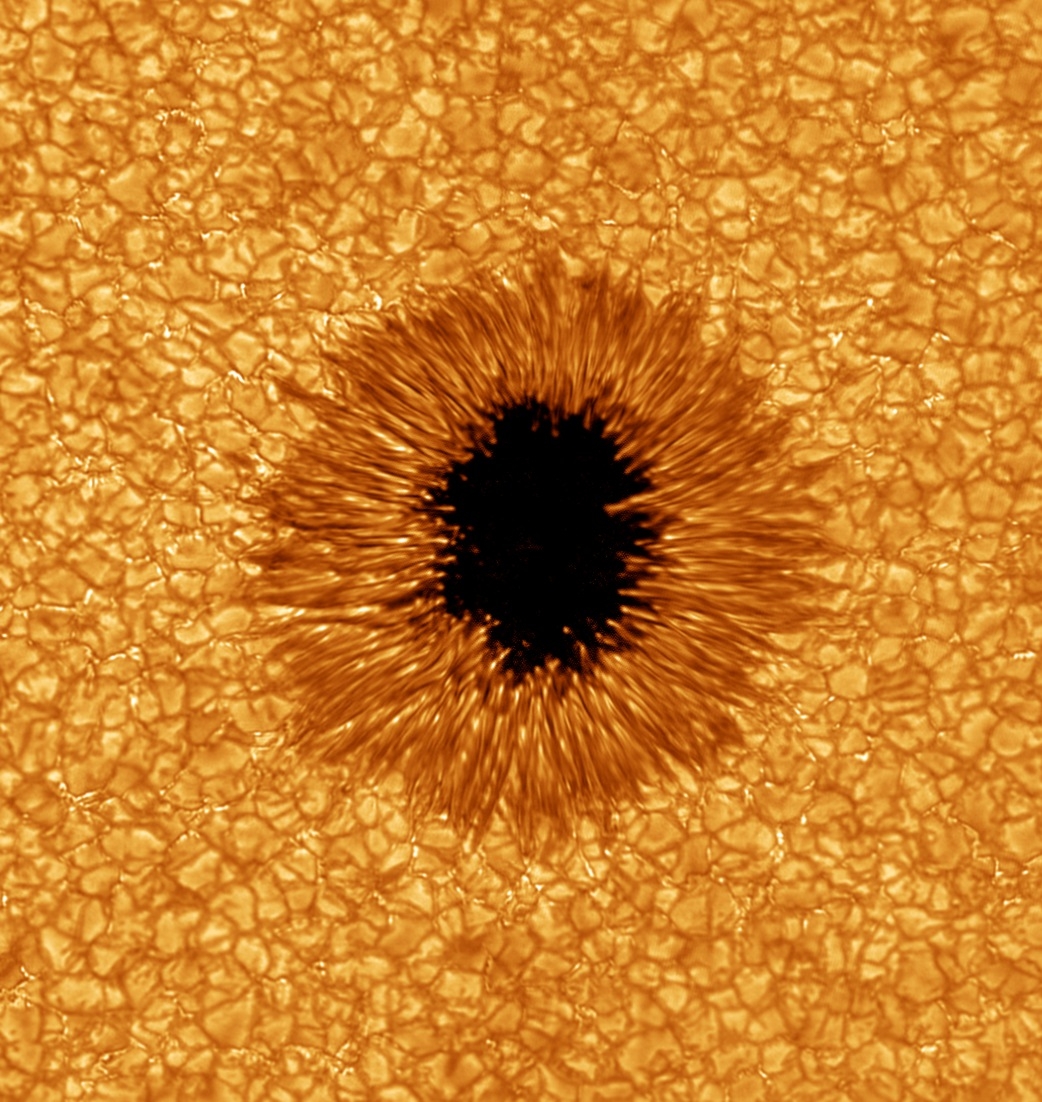
\includegraphics[scale=0.08]{phot.jpg}
			\end{figure}
    \end{column}
\end{columns}

\begin{columns}[b]
    \begin{column}{0.6\textwidth}
		Chromosphere
        \begin{itemize}
					\item not fully collisionally coupled: NLTE, No MHD (frequently not taken into account)
					\item very few spectral lines 
					\item complicated radiative diagostics 
        \end{itemize}
    \end{column}
    \begin{column}{0.5\textwidth}
       % \rule{\textwidth}{0.75\textwidth}
			\begin{figure}[t]
			 \centering
			 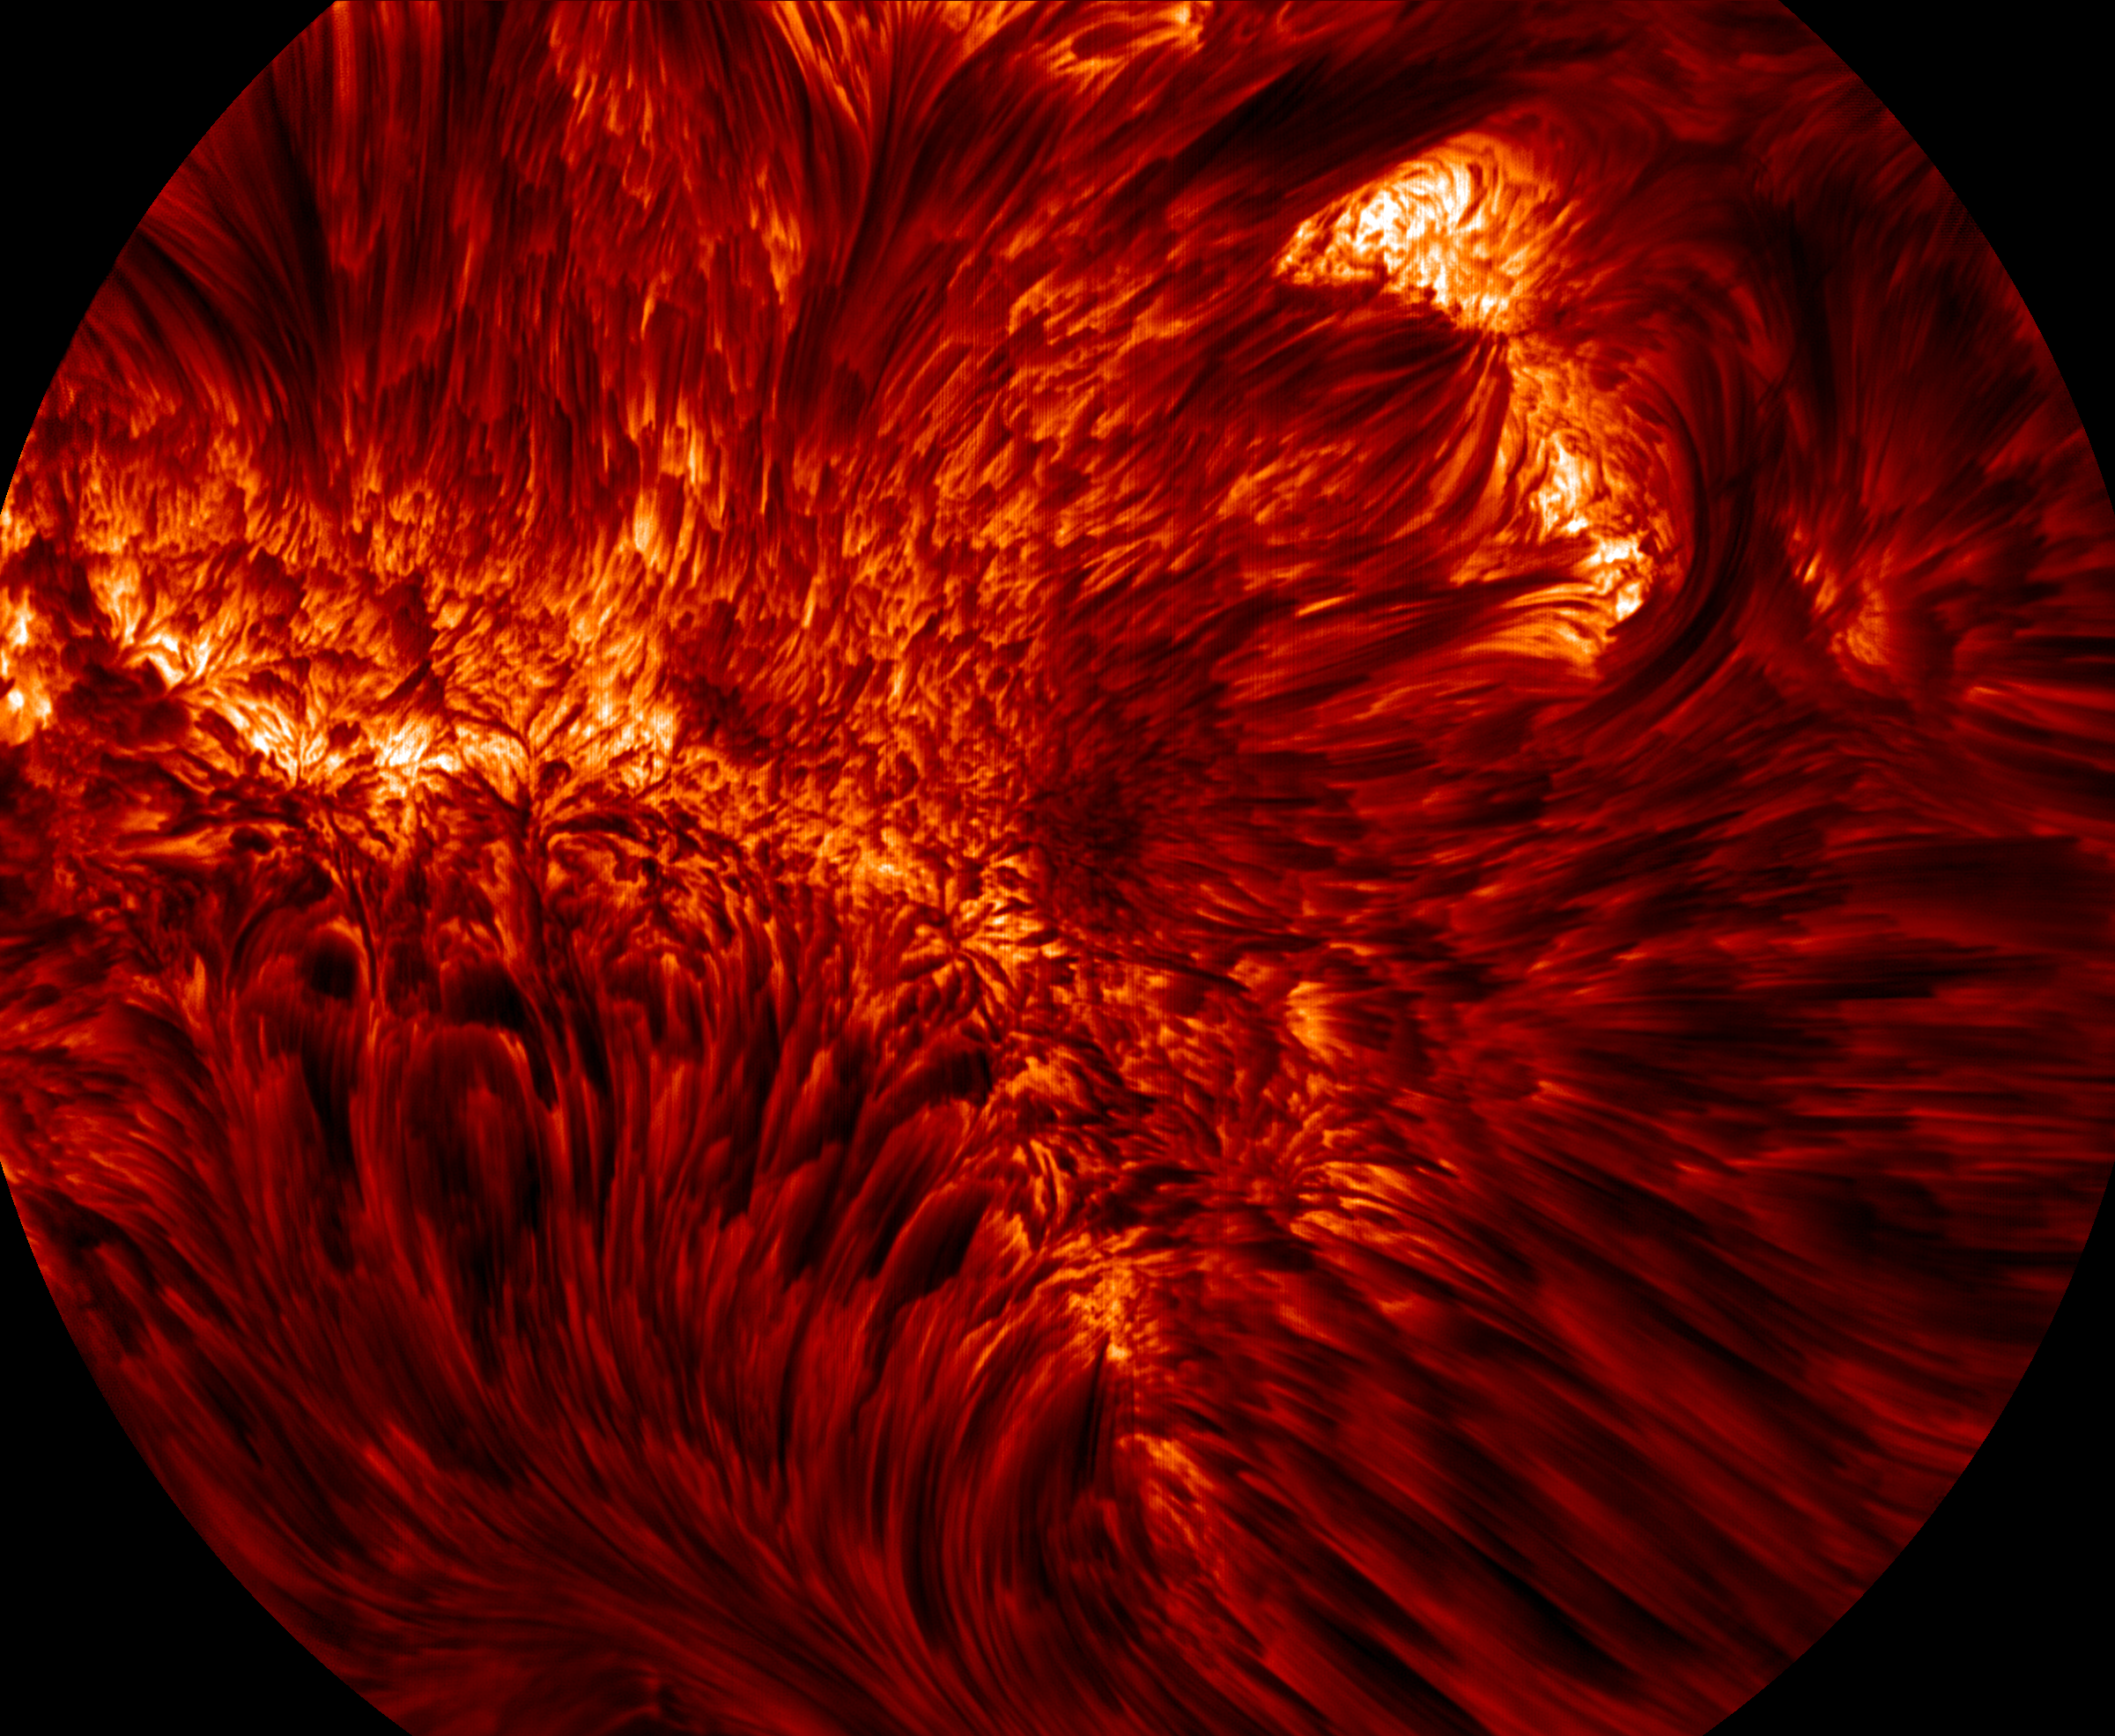
\includegraphics[scale=0.03]{chrom.png}
			\end{figure}
    \end{column}
\end{columns}

\begin{columns}[c]
    \begin{column}{0.6\textwidth}
		Corona
        \begin{itemize}
					\item magnetically dominated 
					\item very low density
					\item all ionized, MHD can be applied
        \end{itemize}
    \end{column}
    \begin{column}{0.5\textwidth}
			\begin{figure}[t]
			 \centering
			 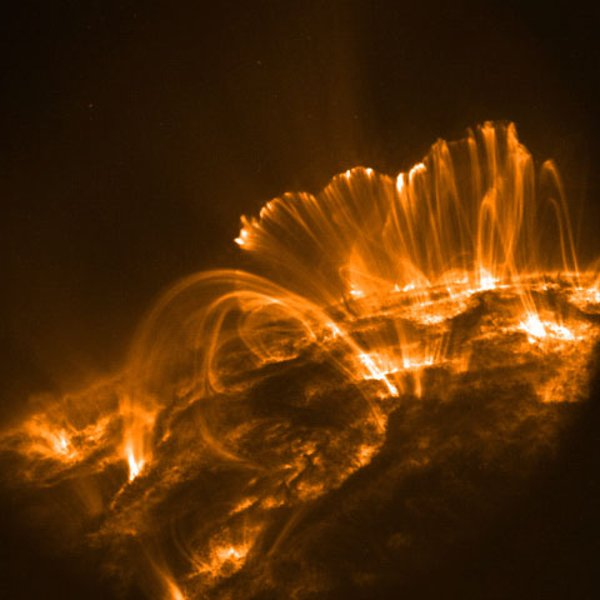
\includegraphics[scale=0.11]{corona.jpg}
			\end{figure}
    \end{column}
\end{columns}

\end{frame}

\begin{frame}{2 fluids model}
\begin{itemize}
\item 13 variables: 10 variables p , $\rho$ and v of the 2 fluids: charges(\_c) and neutrals(\_n) + magnetic field
\item hydrostatic equilibrium(variables: $p_{c0}, p_{n0}, \rho_{c0}, \rho_{n0}$, $\vec{B_0}$), $\vec{v_{c0}}=\vec{v_{n0}}=0$
 
\begin{itemize}
\item charges:
\begin{equation}
\rho_{c0}\vec{g} - \vec{\nabla} p_{c0} + \frac{1}{\mu_0} (\nabla \times \vec{B_0}) \times \vec{B_0} = 0
\end{equation}

\item neutrals:
\begin{equation}
\rho_{n0}\vec{g} - \vec{\nabla} p_{n0}  = 0
\end{equation}

\end{itemize}
\item 13 partial differential equations for the evolution of the perturbation(variables: $p_{c1},p_{n1}, \vec{v_{c1}},\vec{v_{n1}},\rho_{c1}, \rho_{n1}, \vec{B1}$)

\end{itemize}

\end{frame}

\begin{frame}{Boltzmann equation}
\begin{equation}
\frac{\partial f_{\alpha} }{\partial t} + \vec{v} \cdot \vec{\nabla}  f_{\alpha} - \vec{a} \cdot \vec{\nabla_v} f_{\alpha} = (\frac{\partial f_{\alpha}}{\partial t})_{coll}
\end{equation}


with $\alpha \in {i,e,n}$ (charges = e+i)

radiation not taken into account

single ionized H plasma ($n_i = n_e$)

collision terms: $C_{\alpha} \stackrel{\text{not}}{=}  (\frac{\partial f_{\alpha}}{\partial t})_{coll} = C_{\alpha}^{elastic} + C_{\alpha}^{inelastic}$

In order to calculate the $0^{th}$, first and second moment of Boltzmann equation we need to calculate 

$S_\alpha \stackrel{\text{not}}{=} \int_V{C_\alpha d^3\vec{v}}$

$\vec{R_\alpha} \stackrel{\text{not}}{=} \int_V{\vec{v} C_\alpha d^3\vec{v}}$

$M_\alpha \stackrel{\text{not}}{=}  \int_V{v^2 C_\alpha d^3\vec{v}}$

\end{frame}


\begin{frame}{Collision terms(inelastic) }
$C_{\alpha}^{inelastic} = \sum_{\alpha'} {(n_{\alpha'} C_{\alpha'\alpha}^{inelastic} - n_{\alpha} C_{\alpha\alpha'}^{inelastic}}) $

$C_{\alpha\alpha'}^{inelastic} =  \sum_{\beta} {C_{\alpha\alpha',\beta}^{inelastic}  }$

$C_{\alpha\alpha',\beta}^{inelastic} =  \sigma_{\alpha \alpha'} f_{\beta} v_{\beta} $  

where $\sigma_{\alpha \alpha'} = \sigma_{\alpha \alpha'}(v_{\beta}) $  is the collisional cross section of $\alpha$ and $\beta$ 

considering ionization and recombination processes for inelastic collisions:

\textbf{neutrals}:

$C_n^{inelastic} = n_i C^{rec} - n_n C^{ion}$ 

where $C^{ion} \stackrel{\text{not}}{=} C_{ni,e}^{inelastic} = \sigma_{ion} f_e v_e$

$C^{rec} \stackrel{\text{not}}{=} C_{in,e}^{inelastic} = \sigma_{rec} f_e v_e $

$\sigma_{ion}  \stackrel{\text{not}}{=}  \sigma_{ni}= \sigma_{ni} (v_e) $

$\sigma_{rec}  \stackrel{\text{not}}{=}   \sigma_{in}= \sigma_{in} (v_e) $

\textbf{charges}:

$C_c^{inelastic} = -C_n^{inelastic}$ 

\end{frame}


\begin{frame}{Collision terms(inelastic) }

{\color{red} $0^{th}$ moment}

$S_{\alpha\alpha',\beta}^{inelastic} = \int_V{\sigma_{\alpha \alpha'} f_{\beta} v_{\beta} d^3\vec{v} } = n_{\beta} <\sigma_{\alpha \alpha'} v_{\beta} >$  


$S^{ion} = n_e <\sigma_{ion} v_e >$ 

$S^{rec} = n_e <\sigma_{rec} v_e >$


expressions for the collision sections in Leake article:

$<\sigma_{ion} v_e > = \frac{1}{\sqrt{T_e^*}}	2.6 \cdot 10^{-19} m^3/s$

$<\sigma_{rec} v_e > = A \frac{1}{X + \frac{\phi_{ion}}{T_e^*}}	(\frac{\phi_{ion}}{T_e^*})^K  e^{-\frac{\phi_{ion}}{T_e^*} } m^3/s$

where $\phi_{ion} = 13.6 eV$, $T_e^*$ is electron temperature in eV and  they define $A = 2.91 \cdot 10^{-14}, K = 0.39, X = 0.232$


$S_n^{inelastic} = n_i S^{rec} - n_n S^{ion}  $ 




\end{frame}

\begin{frame}{Collision terms(inelastic) }

{\color{red} First moment}

$\vec{R_{\alpha\alpha',\beta}^{inelastic}} = \int_V{\vec{v_\alpha} \sigma_{\alpha \alpha'} f_{\beta} v_{\beta} d^3\vec{v} } $  

$\vec{v_\alpha} = \vec{u_\alpha} + \vec{w_\alpha} $

$\int_V{\vec{w_\alpha} \sigma_{\alpha \alpha'} f_{\beta} v_{\beta} d^3\vec{v} } = 0$

$\int_V{\vec{u_\alpha} \sigma_{\alpha \alpha'} f_{\beta} v_{\beta} d^3\vec{v} } = \vec{u_\alpha} S_{\alpha\alpha',\beta}^{inelastic}$ 
 
$\vec{R_n^{inelastic}} = n_i \vec{u_i} S^{rec} - n_n \vec{u_n} S^{ion}  $ 

{\color{red} Second moment}

$M_{\alpha\alpha',\beta}^{inelastic} = \int_V{v_\alpha^2 \sigma_{\alpha \alpha'} f_{\beta} v_{\beta} d^3\vec{v} }  $

$\int_V{u_\alpha^2 \sigma_{\alpha \alpha'} f_{\beta} v_{\beta} d^3\vec{v} } = u_\alpha^2 S_{\alpha\alpha',\beta}^{inelastic}$

$\int_V{2 \vec{w_\alpha} \vec{u_\alpha} \sigma_{\alpha \alpha'} f_{\beta} v_{\beta} d^3\vec{v} } = 0$
 
$\int_V{w_\alpha^2 \sigma_{\alpha \alpha'} f_{\beta} v_{\beta} d^3\vec{v} } = \frac{3 k_B T_\alpha}{m_\alpha} S_{\alpha\alpha',\beta}^{inelastic} $

$M_n^{inelastic} = n_i u_i^2 S^{rec} - n_n u_n^2 S^{ion} + 3 k_B (\frac{n_i T_i}{m_i} S_{rec} - \frac{n_n T_n}{m_n} S_{ion} ) $ 


\end{frame}

\begin{frame}{Collision terms(elastic)}
$C_{\alpha}^{elastic} = \sum_{\beta} C_{\alpha \beta}^{elastic}$

\textbf{neutrals}:

$C_{n}^{elastic} =  C_{ni}^{elastic}  + C_{ne}^{elastic}$

\textbf{charges}:

$C_{c}^{elastic} =  -C_{n}^{elastic} $

{\color{red} $0^{th}$ moment}

$S_\alpha^{elastic} = \int_V{C_\alpha^{elastic} d^3\vec{v}} = 0 $

{\color{red} First moment}

$\vec{R_\alpha^{elastic} }= \int_V{\vec{v_\alpha} C_\alpha^{elastic} d^3\vec{v}} = \int_V{\vec{w_\alpha} C_\alpha^{elastic} d^3\vec{v}}  $


$\int_V{\vec{w_\alpha} C_{\alpha\beta}^{elastic} d^3\vec{v}}  = n_\alpha \nu_{\alpha\beta} (\vec{u_\beta} - \vec{u_\alpha})$ where $\nu_{\alpha\beta}$ is the collision frequency and 
for  $\alpha \in i,e$ and $\beta=n$ it is expressed as:  $n_\beta \sqrt{\frac{8 k_B T_{\alpha\beta}}{\pi m_{\alpha\beta } }} \Sigma_{\alpha\beta} $

where  $m_{\alpha\beta} = \frac{m_\alpha + m_\beta}{2}$, $T_{\alpha\beta}= \frac{T_\alpha+T_\beta}{2}$ and $\Sigma_{\alpha\beta}$ is the cross section for elastic collisions

($n_\alpha \nu_{\alpha\beta} = n_\beta \nu_{\beta\alpha} $)

$\vec{R_n^{elastic}} =  n_i (\nu_{in} + \nu_{en})  (\vec{u_c} - \vec{u_n})$

\end{frame}

\begin{frame}{Collision terms(elastic)}

$\nu_{in} =n_n \sqrt{\frac{8 k_B T_{ni}}{\pi m_{ni } }} \Sigma_{ni} $, $\nu_{en} = n_n \sqrt{\frac{8 k_B T_{ne}}{\pi m_{ne } }} \Sigma_{ne}$ 

and we use the values: $\Sigma_{ne} = 10^{-19} m^2, \Sigma_{ni} = 5 \cdot 10^{-19} m^2$

{\color{red} Second moment}
$M_\alpha^{elastic} = \int_V{v_\alpha^2 C_\alpha^{elastic} d^3\vec{v}} = 2 \vec{u_\alpha} \int_V{\vec{w_\alpha} C_\alpha^{elastic} d^3\vec{v}} + \int_V{w_\alpha^2 C_\alpha^{elastic} d^3\vec{v}}  $

We neglect the second term for the moment (braginskii 'heat generation') then:

$M_\alpha^{elastic} = 2 \vec{u_\alpha} \vec{R_\alpha^{elastic}}$ 

\end{frame}

\begin{frame}{From Boltzmann equation to the evolution of the perturbations}

transport equation:

\begin{equation}
\frac{\partial (n_{\alpha} <\chi>_{\alpha})}{\partial t} + \nabla \cdot (n_{\alpha} <\chi \vec{v}>_{\alpha} ) - n_{\alpha}<\vec{a} \cdot \vec{\nabla_v} \chi>_{\alpha} = \int_V{\chi (\frac{\partial f_{\alpha}}{\partial t})_{coll} d^3\vec{v} }
\end{equation}

with $\alpha \in n,c$ and  $\chi=m_{\alpha}, m_{\alpha} \vec{v_\alpha}, \frac{1}{2} m_\alpha v_\alpha^2 $ in the Boltzmann transport equation
and using the $0^{th}$, first and second moment of Boltzmann equation
will result in  equations for u=$\rho_\alpha,\rho_\alpha \vec{v_\alpha},\epsilon_\alpha + \frac{1}{2}\rho_\alpha v_\alpha^2 $ 


The equations from the code: 

\begin{equation}
\frac{\partial u}{\partial t} + \nabla \cdot \vec{F_u} = S_u
\end{equation}

$\vec{F_u} = \vec{F_u}^{id} - \vec{F_u}^{diff}, S_u = S_u^{id} + S_u^{coll} + S_u^{diff}$


\end{frame}

\begin{frame}{Diffusivity(artificial)}

Artificial diffusivity coefficients(as in  mancha 1 fluid):

${\nu_u^{diff}}_{x_i} = {\nu_u^{diff\_shock}}_{x_i} + {\nu_u^{diff\_const}}_{x_i} +  {\nu_u^{diff\_var}}_{x_i} $ for $i \in 1,2,3$


${\nu_u^{diff\_shock}}_{x_i} = \textcolor{blue}{\nu_u^{shock}} \cdot max(|\nabla \cdot \vec{v}^{shock}_u|,0.5) \cdot dx_i^2$
for $\nabla \cdot \vec{v}^{shock}_u < 0$  and 0 otherwise where we define

$\vec{v}^{shock}_{\rho_{c1}} = \vec{v}^{shock}_{\epsilon_{c1}}= \vec{v}^{shock}_{\vec{v_{c1}}} = \vec{v_{c1}} $, 
$\vec{v}^{shock}_{\rho_{n1}} = \vec{v}^{shock}_{\epsilon_{n1}}= \vec{v}^{shock}_{\vec{v_{n1}}} = \vec{v_{n1}} $,
$\vec{v}^{shock}_{\vec{B_1}} = \vec{v_c}_{\perp_{\vec{B}}}$ or  $\vec{v_c}_{\perp_{\vec{B_0}}}$

${\nu_u^{diff\_var}}_{x_i}  = \textcolor{blue}{{{\nu_u}^{var}}_{x_i}} \cdot  vflow_u \cdot  dx_i \cdot  hyper_u^{x_i}$

\textbf{hyper} is defined(for example for i = 1):

for each k $\in$ 2..number of points discretized in dimension $x_1$ - 2:

$hyper_u^{x_i}(k,:,:)= \frac{max(\Delta3_u(k-1,:,:),\Delta3_u(k,:,:),\Delta3_u(k+1,:,:))}{max(\Delta1_u(k-1,:,:),\Delta1_u(k,:,:),\Delta1_u(k+1,:,:))}$ where

$\Delta3_u(k,:,:) = |3(u(k+1,:,:) - u(k,:,:)) - (u(k+2,:,:) - u(k-1,:,:)) | $ and $\Delta1_u(k,:,:) = |u(k+1,:,:) - u(k,:,:) | $ 

(we use $T_\alpha$ for $u = \epsilon_\alpha$ when calculating hyper)

$vflow_u = |\vec{v_{c1}}|+ {c_s}_c + v_A$ for u  related to charges and magnetic field and 
$vflow_u = |\vec{v_{n1}}|+ {c_s}_n $ for u  related to neutrals

\end{frame}

\begin{frame}{Diffusivity(artificial)}
${\nu_u^{const\_var}}_{x_i}  = \textcolor{blue}{{{\nu_u}^{const}}_{x_i}} \cdot  vel_u \cdot  dx_i \cdot  \textcolor{blue}{const}$ 

(const is a matrix introduced as a h5 file)

$vel_u =  {c_s}_c + v_A$ for u  related to charges and magnetic field and 
$vel_u =  {c_s}_n $ for u  related to neutrals

\textbf{Fluxes due to the diffusivity}:

${F_{\rho_\alpha}^{diff}}_{x_i} =  {\nu_{\rho_\alpha}^{diff}}_{x_i} \cdot \frac{\partial \rho_{\alpha1}}{\partial x_i}$

${F_{\epsilon_\alpha}^{diff}}_{x_i} =  \rho_\alpha \cdot {\nu_{\epsilon_\alpha}^{diff}}_{x_i} \cdot \frac{\partial T_{\alpha1}}{\partial x_i}$


symmetric diffusivity matrix for the velocities(artificial viscosity):

${F_{\rho_\alpha{v_\alpha}_{x_j}}^{diff}}_{x_i}  = \frac{1}{2} \rho_\alpha \cdot ({\nu_{\rho_\alpha{v_\alpha}_{x_j}}^{diff}}_{x_i} \cdot \frac{\partial {v_\alpha}_{x_j}}{\partial x_i} +  {\nu_{\rho_\alpha{v_\alpha}_{x_i}}^{diff}}_{x_j} \cdot \frac{\partial {v_\alpha}_{x_i}}{\partial x_j} )$

magnetic artificial diffusivity:

$E^{artif\_diff}_{x_1} = {F_{B_{x_3}}^{diff}}_{x_2} - {F_{B_{x_2}}^{diff}}_{x_3}   $,  
$E^{artif\_diff}_{x_2} = {F_{B_{x_1}}^{diff}}_{x_3} - {F_{B_{x_3}}^{diff}}_{x_1}   $,  
$E^{artif\_diff}_{x_3} = {F_{B_{x_2}}^{diff}}_{x_1} - {F_{B_{x_1}}^{diff}}_{x_2}   $  

where 
${F_{B_{x_j}}^{diff}}_{x_i} =  {\nu_{B_{x_j}}^{diff}}_{x_i} \cdot \frac{\partial B_{x_j}}{\partial x_i}$

\end{frame}
\begin{frame}{Continuity equations}
$F_{\rho_{\alpha}}^{id} = \rho_\alpha \vec{v_\alpha} $

$S_n' \stackrel{\text{not}}{=} S_{\rho_n}^{coll} = m_H (n_i S^{rec} - n_n S^{ion} ) = \rho_c S^{rec} - \rho_n S^{ion} $

$S_{\rho_c}^{coll} = -S_n'$
\end{frame}
\begin{frame}{Momentum equations}
symmetric flux matrices:

\textbf{neutrals}

${F_{\rho_{n}{v_n}_{x_i}}^{id}}_{x_j} = \rho_n {v_n}_{x_j} {v_n}_{x_j}  $ 

${F_{\rho_{n}{v_n}_{x_i}}^{id}}_{x_i} = \rho_n {{v_n}_{x_j}}^2 + p_{n1}  $

\textbf{charges}
 
${F_{\rho_{c}{v_c}_{x_i}}^{id}}_{x_j} = \rho_n {v_c}_{x_j} {v_c}_{x_j} - \frac{1}{\mu_0}(B_{x_i 0}B_{x_j 1} + B_{x_j0}B_{x_i1}  + B_{x_i1}B_{x_j1}  ) $ 

${F_{\rho_{c}{v_c}_{x_i}}^{id}}_{x_i} = \rho_n {{v_c}_{x_i}}^2 + p_{c1}  - \frac{1}{2 \mu_0}(B_{x_1 1} (B_{x_1 1} + 2  B_{x_1 0} )+ B_{x_2 1} (B_{x_2 1} + 2  B_{x_2 0} ) + B_{x_3 1} (B_{x_3 1} + 2  B_{x_3 0} ))$

with gravity: $S_{\rho_\alpha \vec{v_\alpha}}^{id} = -\rho_\alpha \vec{g}$

collision sources:

$\vec{R_n'} \stackrel{\text{not}}{=} S_{\rho_n \vec{v_n}}^{coll} =  m_H(n_i \vec{v_c} S^{rec} - n_n \vec{v_n} S^{ion} +\vec{R_n}^{elastic})$

$=\rho_c \vec{v_c} S^{rec} - \rho_n \vec{v_n} S^{ion} +\rho_c \rho_n \alpha^{elastic} (\vec{v_c} - \vec{v_n})$

where $\alpha^{elastic}\stackrel{\text{not}}{=} \frac{1}{m_n^2}(\sqrt{\frac{8 k_B T_{nc}}{\pi m_{in}}} m_{in} \Sigma_{in} +  \sqrt{\frac{8 k_B T_{nc}}{\pi m_{en}}} m_{en} \Sigma_{en})$ 


$S_{\rho_c \vec{v_c}}^{coll} =  -\vec{R_n'} $ 


\end{frame}

\begin{frame}{Momentum equations}
Stiff terms $\rho_c \rho_n \alpha^{elastic} (\vec{v_c} - \vec{v_n})$ calculated as: 

$\frac{\rho_c \rho_n \alpha^{elastic} dt}{1 + \alpha^{elastic}(\rho_c + \rho_n) dt }(\vec{v_c} - \vec{v_n})$


\end{frame}
\begin{frame}{Total energy equations}
$E_c = \epsilon_c + \frac{1}{2} \rho_c v_c^2 + \frac{1}{2\mu_0} B^2$

$E_n = \epsilon_n + \frac{1}{2} \rho_n v_n^2 $

$\vec{F}_{E_{c}}^{id} = (E_c + p_c + \frac{B^2}{2 \mu_0}) \vec{v_c} - \frac{1}{\mu_0} (\vec{v_c}\cdot\vec{B}) \vec{B} $

$\vec{F}_{E_{n}}^{id} = (E_n + p_n) \vec{v_n}  $ 

with gravity: $S_{E_{\alpha}}^{id} = \rho_\alpha \vec{v_\alpha} \vec{g} $

$S_{E_{n}}^{coll}  = {M_n'}^{inelastic}+ m_H \vec{v_n} \vec{R_n}^{elastic}$

where ${M_n'}^{inelastic} \stackrel{\text{not}}{=} m_H (\frac{1}{2} n_i v_c^2 S^{rec} - \frac{1}{2} n_n v_n^2 S^{ion} + \frac{3}{2} k_B (\frac{n_i T_c}{m_i} S_{rec} - \frac{n_n T_n}{m_n} S_{ion}))$ 

$=\frac{1}{2} \rho_c v_c^2 S^{rec} - \frac{1}{2} \rho_n v_n^2 S^{ion} + \frac{3 k_B}{2 m_H}  (\rho_c T_c S_{rec} - \rho_n T_n S_{ion})$

$S_{E_{c}}^{coll} = -{M_n'}^{inelastic} + m_H \vec{v_c} \vec{R_n}^{elastic} $

$\vec{F}_{E_{\alpha}}^{diff}  = \vec{F}_{\epsilon_{\alpha}}^{diff} - \frac{1}{\mu_0} \vec{E}^{diff}  \times \vec{B} + \bar{\bar{F}}_{\rho_{n}\vec{v_\alpha}}^{diff} \cdot \vec{v_\alpha} $ 
\end{frame}

\begin{frame}{Internal energy equations}

internal energy $\epsilon_\alpha = \frac{p_\alpha}{\gamma - 1} $ (If we take into account the ionization energy: $\epsilon_c = \frac{p_c}{\gamma - 1} + n_e \phi_{ion}$)

$\vec{F}_{\epsilon_\alpha}^{id} =  \epsilon_\alpha \vec{v_\alpha}  $ 

$S_{\epsilon_{\alpha}}^{id} = p_\alpha \nabla \cdot \vec{v_\alpha} $

$S_{\epsilon_{n}}^{coll} = S_{E_{n}}^{coll} - \vec{R_n'} \cdot \vec{v_n} + \frac{1}{2} v_n^2 S_n' $ 

$S_{\epsilon_{c}}^{coll} = S_{E_{c}}^{coll} + \vec{R_n'} \cdot \vec{v_c} - \frac{1}{2} v_c^2 S_n' $ 

$S_{\epsilon_c}^{diff}  = \vec{j} \cdot \vec{E}^{diff} $ 

\end{frame}

\begin{frame}{Ohm law and induction equation}

$\vec{E} = - \vec{v} \times \vec{B} - \vec{E}^{artif\_diff} + \vec{E}^{plasma\_diff}$

$\vec{E}^{plasma\_diff} = \nu_c \vec{j} + c_{jb}  \vec{j} \times \vec{B} - c_{jb} \vec{\nabla} p_e  + \nu_A (\vec{v_n} - \vec{v_c})$

where $\nu_C = \frac{m_e(\nu_{ei}+\nu_{en})}{n_e q_e^2}$, $\nu_A= \frac{m_e(\nu_{en}-\nu_{in})}{q_e} $, $c_{jb} = \frac{1}{n_e q_e}$

$\nu_{ei} = n_e \Lambda_C T_{nc}^{-\frac{3}{2}} 3.7\cdot 10^{-6}$, $\Lambda_C = 23.4 - 1.15 log_{10}(n_e)+3.45 log_{10}(\frac{T_{cn}k_B}{q_e})$


evolution of magnetic field:

$\frac{\partial B_1}{\partial t} = - \nabla \times \vec{E}$

\end{frame}
\begin{frame}{Orszag test}
extended from mancha 1 fluid test

no collision terms, variable artificial diffusivity and filtering

\textbf{Initial conditions}:



\end{frame}
\begin{frame}{Acoustic Wave}
extended from mancha 1 fluid test
\textbf{Initial conditions}:

\textbf{hydrostatic equilibrium} in an isothermal gravity stratified atmosphere:

$\vec{B_0}=(0,0,B_{z0})$, $B_{z0} = 50 \cdot 10^{-4}$ T, $\nabla \times \vec{B_0} = 0$

$\frac{\partial p_\alpha}{\partial z} = -\rho_\alpha  g$

we define total pressure at the  base  $p_{00}= p_0(z=0)=1.17 \cdot 10^4$ Pa  and uniform temperature equal for neutrals and charges: $T_0=10000$ K

assuming hydrogen plasma we calculate from Saha equation the pressure of neutrals and charges at the base: $p_{n00}$, $p_{c00}$

we have different pressure scale heights for charges and neutrals: $H_\alpha = \frac{R T_0}{\mu_\alpha g}$ beacuse of different $\mu_c=\frac{1}{2} \mu_n$  and $\mu_n = 1g/mol$ (only H)

we calculate then equilibrium pressure of charges and neutrals: $p_{\alpha0}(z) = p_{\alpha00} exp(-\frac{z}{H_\alpha})$

and density from ideal gas law: $\rho_\alpha = \frac{p_\alpha \mu_\alpha}{R T_0}$
\end{frame}
\begin{frame}{Acoustic Wave}
\textbf{perturbation} - a gaussian shaped(in the xy plane) sound wave generated permanently at the base of the gravity stratified atmosphere:

we specify the amplitude A=100, the period P=50  ($\omega=\frac{2 \pi}{P}$) of the wave, $x_0$, $y_0$, $\sigma_x$, $\sigma_y$ the center and the standard deviation of the gaussian and
 $z_f$ the end of the perturbed region 

the cutoff frequency: ${\omega_c}_\alpha = \frac{\gamma g}{2 {c_s}_\alpha}$

the pressure scale height: $H_\alpha=\frac{{{c_s}_\alpha}^2}{\gamma g}$


\[
k=
 \begin{cases} 
      -\frac{\sqrt{\omega^2 - \omega_c^2}}{{c_s}_\alpha} - \frac{i}{2 H_\alpha}& \omega \ge \omega_c \\
      i(\frac{\sqrt{\omega^2 - \omega_c^2}}{{c_s}_\alpha} - \frac{1}{2 H_\alpha})& \omega < \omega_c 
   \end{cases}
\]

$g = exp(-\frac{(x-x_0)^2}{2 \sigma_x^2} -\frac{(y-y_0)^2}{2 \sigma_y^2} )$

$rr = \frac{1}{\omega}(-k - \frac{i}{H})$

$pp = \frac{1}{\omega}(-k \gamma - \frac{i}{H})$

\end{frame}
\begin{frame}{Acoustic Wave}
$p_{\alpha1}(x,y,z) = A \cdot g(x,y) \cdot {pe_{\alpha0}} |pp| exp(Im(k) (z_f - z)) sin(Re(k) (z_f - z) + \omega t + atan(\frac{Im(pp)}{Re(pp)}))$

$\rho_{\alpha1}(x,y,z) = A \cdot g(x,y) \cdot {\rho_{\alpha0}} |rr| exp(Im(k) (z_f - z)) sin(Re(k) (z_f - z) + \omega t + atan(\frac{Im(rr)}{Re(rr)}))$

$v_{\alpha1}(x,y,z) = A \cdot g(x,y)  exp(Im(k) (z_f - z)) sin(Re(k) (z_f - z) + \omega t))$

in this test we used a Perfectly Matched Layer to avoid reflection at the upper boundary (described in previous version of Mancha) 

for $S^{ion}$ and $S^{rec}$ instead of expression in Leake the derivation of Saha equation in time (only derivating T and not $n_{tot}$):

$\frac{\partial n_e}{\partial t} = 
((\frac{2  \pi  m_e  k_B}{h^2})^{1.5} \frac{\partial T_{cn}}{\partial t} exp(-\frac{\phi_{ion}} {k_B T_{cn}})
      (1.5  \sqrt{T_{cn}}  + \frac{\phi_{ion}}{k_B T_{cn}^2 } ) 
     ( \frac{2 A+ n_{tot}}{2 \sqrt{A^2 + A n_{tot}} } - 1)
       min(\frac{dt}{te\_relaxation\_timescale},1)$

				where $A = (\frac{2  \pi  m_e  k_B  T_{cn}}{h^2})^{1.5}  exp(-\frac{\phi_{ion}} { (k_B  T_{cn}})$

and te\_relaxation\_timescale is the relaxation time for saha: parameter set to 10 in this test


\end{frame}
\begin{frame}{Acoustic Wave}
     where($\frac{\partial n_e}{\partial t} <0$) $S^{rec} = -\frac{1}{\rho_c} \frac{\partial n_e}{\partial t} $, $S^{ion} = 0 $

     elsewhere $S^{ion} = \frac{1}{\rho_n} \frac{\partial n_e}{\partial t} $, $S^{rec} = 0 $

\end{frame}
\begin{frame}{Reconnection}
\end{frame}
\end{document}
